\section{Elementy interfejsu użytkownika (8)}

\subsection{Wykresy funkcji (1)} 

      Napisać program, który tworzy okno i w jego obszarze roboczym rysuje wykresy funkcji $f(x) = |x|$ i 
\label{wykres_z_osiami}	  
      $f(x) = x^2$ (z osiami). Oba wykresy powinny być narysowane różnymi kolorami i różnymi stylami pędzli.
      
      Wykresy powinny automatycznie dopasowywać się do nowych rozmiarów okna podczas skalowania okna.
      
      [{\bf 1p}]

\subsection{Poruszające się kółko (1)} 

      Napisać program, który w obszarze roboczym okna pokaże poruszające się i odbijające się od ramki okna kółko. 
\label{poruszajace_kolko}
      
      Kółko powinno poprawnie reagować na skalowanie rozmiarów okna przez użytkownika.
      
      [{\bf 1p}]

\subsection{Okno dialogowe (2)} 
      
      Napisać program, który odtworzy następujący wygląd okna z rysunku \ref{r1}.
\label{okno_dialogowe}

	\begin{figure}
	\begin{center}
	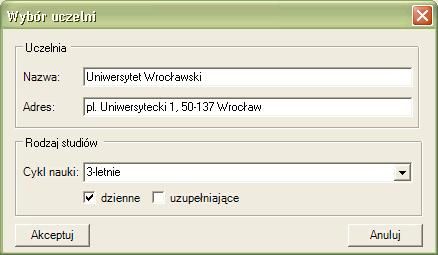
\includegraphics[width=0.75\textwidth]{z1_01}
	\end{center}
	\caption{Wygląd okna do zadania [\ref{okno_dialogowe}]}
	\label{r1}
	\end{figure}

      Okno zawiera dwie ramki grupujące ({\em Group Box}). Pierwsza ramka zawiera dwa pola tekstowe
      ({\em Edit Box}), druga zawiera pole wyboru ({\em Combo Box}) oraz dwa przyciski stanu ({\em Check Box}).

      Lista rozwijalna pola wyboru powinna być wypełniona przykładowymi nazwami.

      Po wybraniu przez użytkownika przycisku {\bf Akceptuj}, wybór powinien zostać zaprezentowany w oknie
      informacyjnym (rysunek \ref{r2}).

      	\begin{figure}
	\begin{center}
	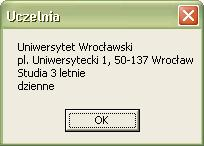
\includegraphics[width=0.25\textwidth]{z1_02}
	\end{center}
	\caption{Informacja dla użytkownika do zadania [\ref{okno_dialogowe}]}
	\label{r2}
	\end{figure}

      Naciśnięcie przycisku {\bf Anuluj} powinno zakończyć program.
      
      {\em Uwaga! Formanty potomne należy inicjować bezpośrednio przez {\tt CreateWindow}. Komunikat w oknie informacyjnym zależy oczywiście od
      danych wprowadzonych przez użytkownika na formularzu głównym}.
      
      [{\bf 2p}]

\subsection{Szablon okna dialogowego (2)} 
      
      Powtórzyć funkcjonalność programu z zadania [\ref{okno_dialogowe}] używając tym razem 
\label{szablon_okna}	  
	  edytora zasobów i wbudowanej w niego wizualnego funkcji wizualnej edycji szablonu okna do zbudowania interfejsu użytkownika. 
	  
      {\em Uwaga! W przypadku tworzenia okna z szablonu zapisanego w zasobach, zmiast {\tt RegisterClass}, {\tt CreateWindow} i jawnej pętli obsługi komunikatów użyć funkcji {\tt DialogBox}}.

      [{\bf 2p}]

\subsection{Wybrane składniki {\tt Common Controls} (2)}

      Napisać program, który zademonstruje działanie trzech wybranych komponentów biblioteki formantów Common Controls
\label{common_controls}	  
      (ListView, TreeView, Progress Bar, Status Bar, Tool Bar, itd.). Demonstracja ma polegać
      na obsłudze kilku wybranych właściwości komponentów (na przykład wypełnieniu ListView kilkoma
      elementami, zmianie wartości i stylu Progress Bara itp.). 
      
      [{\bf 2p}]
            
